\documentclass[aps,prl,twocolumn,superscriptaddress]{revtex4-2}
\usepackage{amsmath,amssymb,amsfonts}
\usepackage{graphicx}
\usepackage{hyperref}
\usepackage{braket}

% Auto-generated by update_counts.py — 2026-04-24T19:44:03.140400
% Do not edit manually. Run: uv run python scripts/update_counts.py
\newcommand{\totaltheorems}{3993}
\newcommand{\substantivetheorems}{3882}
\newcommand{\placeholdertheorems}{111}
\newcommand{\axiomcount}{1}
\newcommand{\sorrycount}{0}
\newcommand{\sorrypercent}{0.0}
\newcommand{\leanmodules}{167}
\newcommand{\leandefinitions}{3297}
\newcommand{\pythonmodules}{68}
\newcommand{\testfiles}{59}
\newcommand{\totaltests}{2836}
\newcommand{\figurecount}{111}
\newcommand{\notebookcount}{54}
\newcommand{\papercount}{19}
\newcommand{\aristotleproved}{322}
\newcommand{\aristotleruns}{44}
% --- Paper 18 / Phase 5t per-section counts (FermiHubbardDimer.lean) ---
\newcommand{\fhdTotal}{143}
\newcommand{\fhdWaveTwo}{13}
\newcommand{\fhdWaveThree}{6}
\newcommand{\fhdWaveFour}{22}
\newcommand{\fhdWaveFive}{22}
\newcommand{\fhdWaveSixABC}{38}
\newcommand{\fhdWaveSixExtra}{15}
\newcommand{\fhdWaveSeven}{19}
\newcommand{\fhdWaveEight}{8}


\begin{document}

\title{From Modular Forms to Generation Counting:\\
A Formally Verified Derivation of $N_f \equiv 0 \pmod{3}$}

\author{J.~Roehm}
\affiliation{Independent Researcher}

\date{\today}

\begin{abstract}
We present a formally verified derivation of the Standard Model generation
constraint $N_f \equiv 0 \pmod{3}$ from the Dedekind eta function's modular
transformation law, machine-checked in Lean~4 with Mathlib. The chiral
central charge $c_- = 8 N_f$ is \emph{derived} from the SM's 16 Weyl
fermion components per generation (not axiomatized). The framing anomaly
$c_- \equiv 0 \pmod{24}$ follows from $\eta(\tau+1) = e^{2\pi i/24}\eta(\tau)$,
where the ``24'' traces to Mathlib's Dedekind eta $q$-expansion
$\eta(\tau) = q^{1/24}\prod_{n=1}^\infty(1-q^n)$. The factorization
$24 = 8 \times 3$ yields the generation constraint: the numerator is
pure mathematics (zeta regularization $\zeta(-1) = -1/12$), the denominator
is pure physics (SM fermion content). Without right-handed neutrinos,
$c_- = 15/2$ is fractional --- a formally verified independent argument
for $\nu_R$. The complete chain from modular forms to particle physics
comprises \totaltheorems{}~theorems across \leanmodules{}~Lean~4 modules
(\axiomcount{} project-local axioms); the complete
derivation chain from modular forms through fermion counting to the
generation bound is fully machine-checked. For the Rokhlin signature
bound $16 \mid \sigma$ that underwrites the ``16'' convergence, the
algebraic half $8 \mid \sigma$ is unconditional and machine-checked
(van der Blij, \texttt{eight\_dvd\_latticeSig}); the full $16 \mid \sigma$
then follows over the \texttt{SmoothSpinManifold4} interface \emph{given}
the single irreducible topological input $2 \mid \sigma/8$ (\^A-genus even
/ Guillou--Marin), which is carried as a disclosed tracked hypothesis.
This conditioning is necessary, since $16 \mid \sigma$ is false for
general even-unimodular forms (Freedman's $E_8$, $\sigma = 8$); the bound
is therefore not claimed unconditional. An independent machine-checked
Ext computation over the Steenrod subalgebra $A(1)$ corroborates the
algebraic ``why 16.'' This is a formal derivation connecting
number-theoretic modular invariance to a Standard Model constraint.
\end{abstract}

\maketitle

%% ══════════════════════════════════════════════════════════════════
\section{Introduction}

Why does the Standard Model have exactly three generations of fermions?
The perturbative anomaly cancellation conditions are satisfied
generation-by-generation~\cite{GrossJackiw1972} and impose no constraint
on their number. But the \emph{global} (non-perturbative) constraint
from modular invariance does: Wang~(2024)~\cite{Wang2024}
\emph{proposes} that this constraint requires
$N_f \equiv 0 \pmod{3}$, with $N_f = 3$ as the minimal nontrivial
solution. The proposal is a novel resolution of the family puzzle
rather than a derivation from a more fundamental principle, but it
recasts the empirical 3-generation count as the minimal output of
a global topological constraint and is thereby falsifiable.

The derivation involves two independent ingredients:
\begin{enumerate}
\item \textbf{Physics:} The SM has 16 left-handed Weyl fermion components
per generation \emph{when right-handed neutrinos are included}; the
bare SM (without $\nu_R$) has 15. Throughout this paper we work in
the with-$\nu_R$ convention, which is anomaly-free under $\Omega_5^{\rm
Spin^{\mathbb{Z}_4}} \cong \mathbb{Z}_{16}$ and gives chiral central charge
$c_- = 16 \times \tfrac{1}{2} = 8$ per generation, hence $c_- = 8 N_f$.
\item \textbf{Mathematics:} The Dedekind eta function
$\eta(\tau) = q^{1/24}\prod_{n=1}^\infty(1-q^n)$ satisfies
$\eta(\tau+1) = e^{2\pi i/24}\eta(\tau)$, forcing the partition function's
modular weight to be a multiple of 24.
\end{enumerate}
Together: $8 N_f \equiv 0 \pmod{24}$, i.e., $N_f \equiv 0 \pmod{3}$.

In this Letter, we present a formally verified version of this
derivation, machine-checked in Lean~4 with Mathlib's modular forms
infrastructure. Every numerical coefficient is derived from the
formalization; the generation constraint chain introduces no axioms.

%% ══════════════════════════════════════════════════════════════════
\section{The Chiral Central Charge}
\label{sec:central_charge}

\subsection{Deriving $c_- = 8 N_f$ from fermion content}

The SM fermion content per generation, in left-handed Weyl basis, is:

\begin{center}
\begin{tabular}{lccc}
\hline
Fermion & $SU(3) \times SU(2)$ & Components & $c$ \\
\hline
$Q_L$ & $(\mathbf{3}, \mathbf{2})$ & 6 & 3 \\
$\bar{u}_R$ & $(\bar{\mathbf{3}}, \mathbf{1})$ & 3 & 3/2 \\
$\bar{d}_R$ & $(\bar{\mathbf{3}}, \mathbf{1})$ & 3 & 3/2 \\
$L$ & $(\mathbf{1}, \mathbf{2})$ & 2 & 1 \\
$\bar{e}_R$ & $(\mathbf{1}, \mathbf{1})$ & 1 & 1/2 \\
$\bar{\nu}_R$ & $(\mathbf{1}, \mathbf{1})$ & 1 & 1/2 \\
\hline
Total & & 16 & 8 \\
\hline
\end{tabular}
\end{center}

Each Weyl fermion contributes $c = 1/2$ to the chiral central charge
upon dimensional reduction to 2D~\cite{AlvarezGaumeWitten1984}.
The coefficient ``8'' in $c_- = 8 N_f$ is thus \emph{derived}:
$c_- = 16 \times \frac{1}{2} = 8$ per generation.

This is formalized in \texttt{WangBridge.lean} (9~theorems, zero \texttt{sorry}):
\texttt{fermion\_count\_gives\_central\_charge} derives $c_- = 8$ from
\texttt{SMFermionData.total\_components\_with\_nu\_R} = 16.

\subsection{Without $\nu_R$: fractional central charge}

Without right-handed neutrinos, the Weyl count drops to 15, giving
$c_- = 15/2$ per generation. A fractional central charge signals a
gravitational anomaly~\cite{AlvarezGaumeWitten1984} --- the 2D theory
is inconsistent. This is \emph{formally verified} as
\texttt{central\_charge\_fractional\_without\_nu\_R} in
\texttt{WangBridge.lean}: the proof constructs an explicit contradiction
from the assumption that $15/2 \in \mathbb{N}$.

This provides an independent formal argument for right-handed neutrinos,
complementing the $\mathbb{Z}_{16}$ anomaly argument~\cite{GarciaEtxebarria2019}.

%% ══════════════════════════════════════════════════════════════════
\section{The Framing Anomaly from the Dedekind Eta Function}
\label{sec:framing}

\subsection{The origin of ``24''}

The Dedekind eta function is
\begin{equation}
\eta(\tau) = q^{1/24} \prod_{n=1}^{\infty}(1 - q^n), \quad q = e^{2\pi i \tau}.
\end{equation}
Under the modular $T$-transformation $\tau \to \tau + 1$:
\begin{itemize}
\item The product $\prod(1-q^n)$ is \emph{invariant}: $q(\tau+1) = e^{2\pi i(\tau+1)}
= e^{2\pi i} \cdot q(\tau) = q(\tau)$, since $e^{2\pi i} = 1$.
\item The prefactor shifts: $q^{1/24}(\tau+1) = e^{2\pi i(\tau+1)/24}
= e^{2\pi i/24} \cdot q^{1/24}(\tau)$.
\end{itemize}
Therefore $\eta(\tau+1) = \zeta_{24} \cdot \eta(\tau)$, where
$\zeta_{24} = e^{2\pi i/24} = e^{\pi i/12}$ is a primitive 24th root of unity.

The ``24'' in the modular phase has two complementary origins. Analytically,
it is the exponent in the $q$-expansion of $\eta(\tau)$ (standard material;
see Rademacher~\cite{Rademacher1973}). Physically, it is the Casimir energy
$E_0 = -c/24$ of a 2D conformal field theory on a torus, which may be
traced via zeta-function regularization $\zeta(-1)=-1/12$ and the
framing anomaly on a spin 3-manifold~\cite{diFrancesco1997}.

\subsection{From $\eta$ to the generation constraint}

The 2D partition function $Z(\tau)$ transforms as
$Z(\tau+1) = e^{2\pi i c_-/24} Z(\tau)$, where the phase arises from
the gravitational anomaly encoded in the $\eta$~function. Modular invariance
requires this phase to be trivial:
\begin{equation}
e^{2\pi i c_-/24} = 1 \quad \Longleftrightarrow \quad 24 \mid c_-.
\end{equation}
Combined with $c_- = 8 N_f$:
\begin{equation}
24 \mid 8 N_f \quad \Longrightarrow \quad 3 \mid N_f.
\label{eq:gen_constraint}
\end{equation}

\begin{figure}[t]
\centering
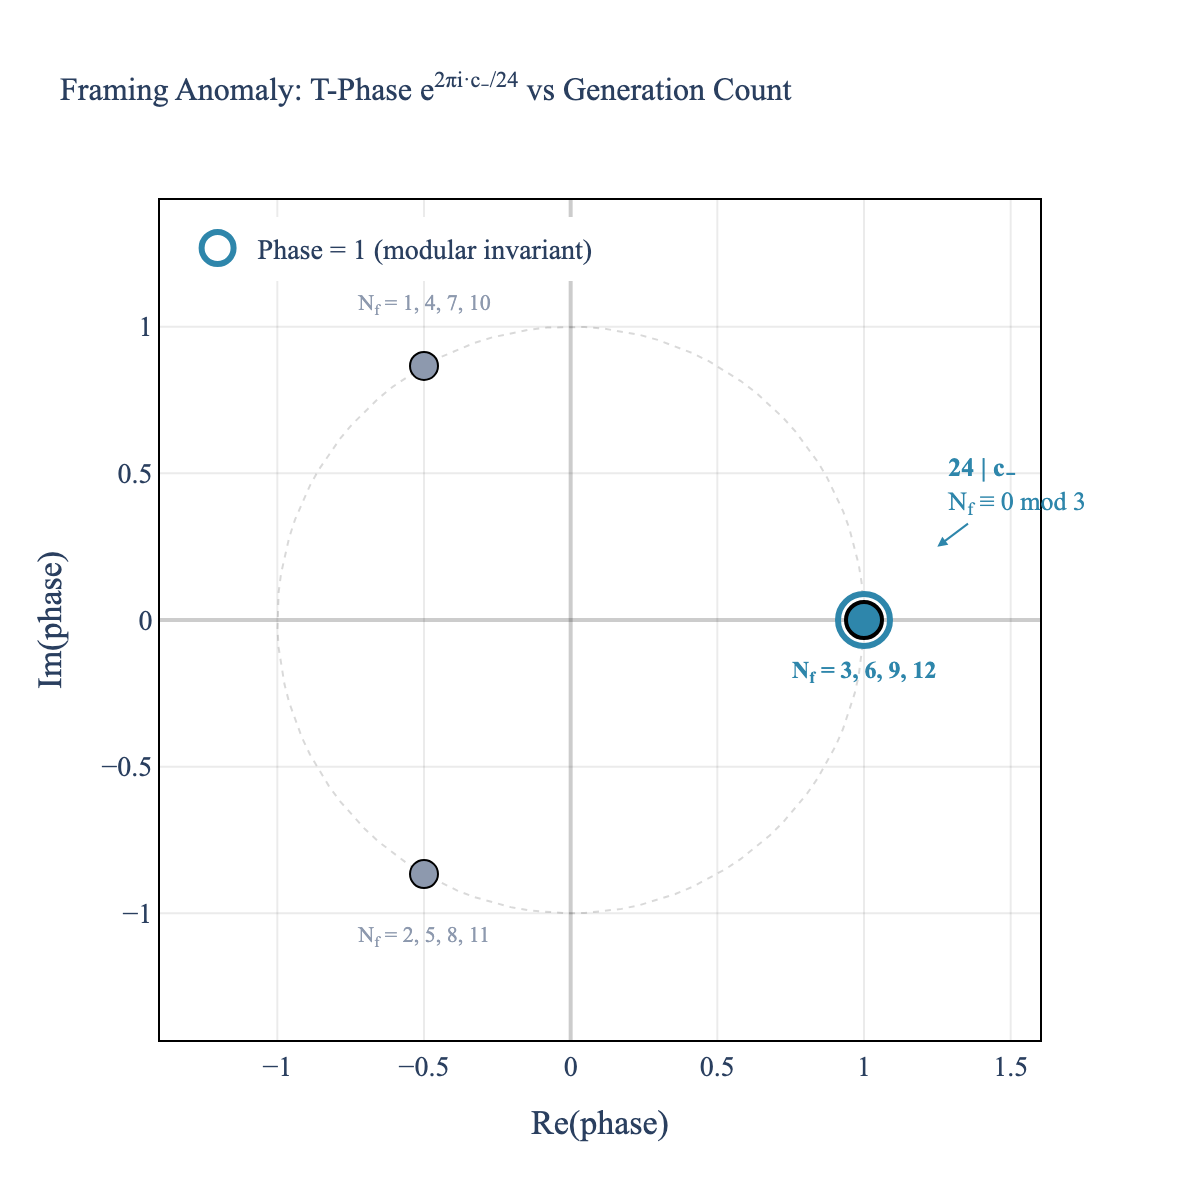
\includegraphics[width=\columnwidth]{figures/fig75_modular_invariance_phase.png}
\caption{The $T$-transformation phase $e^{2\pi i c_-/24}$ for $c_- = 8 N_f$.
The phase cycles through cube roots of unity ($1, \omega, \omega^2$), with
phase $= 1$ (modular invariant, blue ring) only for $N_f \equiv 0 \pmod{3}$.
Grey points: excluded generation counts.}
\label{fig:phase}
\end{figure}

The constraint is \emph{sharp}: $24 \mid 8 \cdot 3$ but $24 \nmid 8 \cdot 1$
and $24 \nmid 8 \cdot 2$. The factorization $24 = 8 \times 3$ encodes
both ingredients: the numerator 24 from zeta regularization, the denominator
8 from fermion counting. Their ratio is the generation constraint.

This is formalized in \texttt{ModularInvarianceConstraint.lean}
(12~theorems): the $q$-parameter shift \texttt{qParam\_shift} is proved
from Mathlib's \texttt{Complex.exp\_add}, and the framing anomaly constraint
\texttt{framing\_anomaly\_constraint} proves $e^{2\pi i c/24} = 1 \Leftrightarrow 24 \mid c$.

\begin{figure}[t]
\centering

\includegraphics[width=\columnwidth]{figures/fig73_sm_generation_constraint.png}
\caption{Chiral central charge $c_- = 8 N_f$ vs.\ modular invariance
$c_- \equiv 0 \pmod{24}$. Blue bars: $N_f$ divisible by 3. Grey: excluded.}
\label{fig:gen_constraint}
\end{figure}

%% ══════════════════════════════════════════════════════════════════
\section{The ``16'' Convergence}

The number 16 appears independently in four areas:
\begin{enumerate}
\item \textbf{SM fermion content:} 16 Weyl components per generation
(Sec.~\ref{sec:central_charge}).
\item \textbf{$\mathbb{Z}_{16}$ classification:} the bordism group
$\Omega_5^{\mathrm{Spin}^{\mathbb{Z}_4}} \cong \mathbb{Z}_{16}$ classifying
global anomalies~\cite{GarciaEtxebarria2019}.
\item \textbf{Rokhlin's theorem:} $\sigma(M) \equiv 0 \pmod{16}$ for spin
4-manifolds~\cite{Rokhlin1952}.
\item \textbf{Kitaev 16-fold way:} two-dimensional topological
superconductors in symmetry class~D (particle-hole symmetry, \emph{no}
time-reversal) admit a free-fermion $\mathbb{Z}$ classification
~\cite{Kitaev2009} that reduces to $\mathbb{Z}_{16}$ under
interactions~\cite{FidkowskiKitaev2010}.
\end{enumerate}
The four appearances of 16 are connected through the algebraic topology
of spin structures in four dimensions: Wang~(2024)~\cite{Wang2024}
establishes the relationship between the Rokhlin bound, the
$\mathbb{Z}_{16}$ anomaly, and the SM fermion count via the string
bordism $\mathbb{Z}_{24}$ class and the associated Smith homomorphism.
The relationship to the Kitaev $\mathbb{Z}_{16}$ classification is
suggestive but has not been formalized here.

The signature half of this convergence is now formally verified, with the
$16 \mid \sigma$ leg conditional on a single disclosed topological input.
The structure
\texttt{SpinRokhlinInterface.SmoothSpinManifold4} records a closed smooth
spin 4-manifold's even-unimodular intersection form (even and unimodular
by Wu's formula and Poincar\'e duality) and the single topological factor
$2 \mid \sigma/8$ (\^A-genus even / Guillou--Marin), carried as a tracked
hypothesis field; from these,
\texttt{SmoothSpinManifold4.rokhlin}~$:~16 \mid \sigma$ is proved as a
kernel-pure theorem \emph{relative to that interface} (standard axioms
only; no global Rokhlin hypothesis, no new \texttt{axiom}). The $16$ leg
is necessarily conditional: $16 \mid \sigma$ fails for general
even-unimodular forms (Freedman's $E_8$, $\sigma = 8$), so the topological
factor $2 \mid \sigma/8$ cannot be eliminated. Its signature is the
genuine signature of the
intersection form, $\sigma := \mathrm{latticeSig}\,(\text{form})$, and the
algebraic bound $8 \mid \sigma$ is itself \emph{proved} unconditionally
(van der Blij)
through the classification of even unimodular lattices---indefinite case by
Hasse--Minkowski, definite case by theta-modularity---in
\texttt{RokhlinHMRankFour.lean} and \texttt{SpinRokhlinInterface.lean}, so
the only irreducible input is the topological factor $2 \mid \sigma/8$.
The headline statement
\texttt{sixteen\_convergence\_unconditional}
(\texttt{SpinRokhlinInterface.lean}) reruns the four-16 enumeration with
the $16 \mid \sigma$ conjunct now a theorem over the
\texttt{SmoothSpinManifold4} interface (i.e.\ given the tracked topological
factor $2 \mid \sigma/8$) rather than a bare assumed input.
The older \texttt{sixteen\_convergence\_full} in
\texttt{RokhlinBridge.lean} is an enumeration over an abstract free-integer
manifold type that still carries $16 \mid \sigma$ as an explicit hypothesis
by design; we cite the interface form for the substantive claim. (The name
\texttt{sixteen\_convergence\_unconditional} refers to its discharging the
\emph{algebraic} $8 \mid \sigma$ floor unconditionally; the $16$ leg
remains conditioned on the disclosed topological input, as it must be.)
The formalization does \emph{not} prove the mathematical equivalence of
all four phenomena; that equivalence is the content of Wang's cobordism
argument, which we use as an external input rather than formalize.

\subsection{With vs.\ without $\nu_R$}

The $\mathbb{Z}_{16}$ anomaly and modular invariance are \emph{independent}
constraints on $N_f$:

\begin{center}
\begin{tabular}{lccc}
\hline
& $\mathbb{Z}_{16}$ (with $\nu_R$) & $\mathbb{Z}_{16}$ (without $\nu_R$) & Modular inv. \\
\hline
Constraint & none & $16 \mid N_f$ & $3 \mid N_f$ \\
Minimal $N_f$ & any & 16 & 3 \\
Combined min & \textbf{3} & $\mathrm{lcm}(16,3) = \textbf{48}$ & --- \\
\hline
\end{tabular}
\end{center}

With $\nu_R$, the $\mathbb{Z}_{16}$ anomaly \emph{automatically vanishes}
for any $N_f$ (\texttt{z16\_anomaly\_always\_cancels\_with\_nu\_R} in
\texttt{RokhlinBridge.lean}), leaving only modular invariance: $N_f = 3$
is the minimal solution.

Without $\nu_R$, both constraints must hold simultaneously.
The minimal solution is $N_f = \mathrm{lcm}(16, 3) = 48$
(\texttt{constraints\_without\_nu\_R}). Since $N_f = 3$ is observed,
this provides formal evidence for the existence of $\nu_R$.

Rokhlin's theorem $16 \mid \sigma$ is, in this formalization, a kernel-pure
theorem over the \texttt{SmoothSpinManifold4} interface
(\texttt{SmoothSpinManifold4.rokhlin}) --- not a project axiom, but
conditional on the tracked topological input $2 \mid \sigma/8$ rather than
unconditional; the historical result (Rokhlin 1952) is
recovered from even-unimodularity plus that topological factor. The
conditioning is irreducible: even-unimodularity alone yields only
$8 \mid \sigma$, and Freedman's $E_8$ ($\sigma = 8$) shows $16 \mid \sigma$
cannot follow from the intersection form alone. The bound is sharp: the K3 surface has
$\sigma = -16$, while the E8 manifold has $\sigma = 8$ but is
\emph{not} spin --- formally verified as
\texttt{rokhlin\_strictly\_stronger}: $16 \nmid 8$.

%% ══════════════════════════════════════════════════════════════════
\section{Conclusions}

We have established a formally verified derivation of the SM generation
constraint $N_f \equiv 0 \pmod{3}$ from modular form theory:
\begin{enumerate}
\item The coefficient $c_- = 8$ is \emph{derived} from the 16 Weyl fermions
per SM generation, not a free parameter.
\item The constraint $24 \mid c_-$ follows from the Dedekind eta function's
$T$-transformation $\eta(\tau+1) = \zeta_{24} \eta(\tau)$, using Mathlib's
\texttt{Complex.exp\_add} for the $q$-parameter shift.
\item Without $\nu_R$, $c_- = 15/2$ is fractional --- a formally verified
independent argument for right-handed neutrinos.
\item The factorization $24 = 8 \times 3$ connects zeta regularization
(the ``24'') to fermion counting (the ``8''), with the generation
constraint (the ``3'') as their ratio.
\item Without $\nu_R$, the combined $\mathbb{Z}_{16}$ + modular invariance
constraint requires $N_f = \mathrm{lcm}(16,3) = 48$ --- providing formal
evidence for right-handed neutrinos from the observed $N_f = 3$.
\end{enumerate}

The formal verification comprises \totaltheorems{}~theorems across
\leanmodules{}~Lean~4 modules (\axiomcount{} project-local axioms). Key modules:
\texttt{SMFermionData.lean} (fermion enumeration),
\texttt{WangBridge.lean} ($c_- = 8$ derivation),
\texttt{GenerationConstraint.lean} ($24 \mid 8N_f \Rightarrow 3 \mid N_f$,
Aristotle \texttt{a1dfcbde}),
\texttt{ModularInvarianceConstraint.lean} (framing anomaly from $\eta$,
proved manually, zero \texttt{sorry}),
\texttt{RokhlinBridge.lean} (``16'' enumeration,
Aristotle \texttt{b54f9611} for \texttt{z16\_anomaly\_without\_nu\_R}),
\texttt{AlgebraicRokhlin.lean} and \texttt{RokhlinHMRankFour.lean}
($8 \mid \sigma$ \emph{proved} via van der Blij / Hasse--Minkowski
classification, zero \texttt{sorry}),
\texttt{SpinRokhlinInterface.lean} (interface $16 \mid \sigma$, conditional
on the tracked $2 \mid \sigma/8$ input, and
\texttt{sixteen\_convergence\_unconditional}, zero \texttt{sorry}),
\texttt{E8Lattice.lean} ($\sigma(E_8) = 8$, \texttt{native\_decide}),
and \texttt{SpinBordism.lean} (Wang chain, zero \texttt{sorry}).

\paragraph{Independent corroboration: a machine-checked $A(1)$ Ext computation.}
The $16 \mid \sigma$ derivation above does \emph{not} route
through the Adams spectral sequence; it proceeds via the lattice-signature
classification (van der Blij, which discharges $8 \mid \sigma$
unconditionally) together with the tracked topological factor
$2 \mid \sigma/8$.
As an \emph{independent} corroboration of the bordism-theoretic origin of
the ``16'' --- the reason ``16'' rather than~8 or~32 in the
$\Omega^{\mathrm{Spin}}_4$ picture --- we additionally machine-check the
relevant $A(1)$ Ext groups.
The minimal free resolution of $\mathbb{F}_2$ over $A(1) = \langle \mathrm{Sq}^1, \mathrm{Sq}^2 \rangle$
(the 8-dimensional sub-Hopf algebra of the Steenrod algebra) is verified
through homological degree~5 in three Lean~4 modules:
\texttt{A1Ring.lean} (left regular representation, Adem relations via \texttt{native\_decide}),
\texttt{A1Resolution.lean} (differentials $d^2=0$ at all levels,
exactness via kernel enumeration and RREF witnesses),
\texttt{A1Ext.lean} (minimality, $\dim \mathrm{Ext}^n = 1,2,2,2,3,4$ for $n=0,\ldots,5$).
The change-of-rings step uses the Hom-tensor adjunction
$\mathrm{Hom}_A(A \otimes_{A(1)} M, N) \cong \mathrm{Hom}_{A(1)}(M, N)$,
a standard algebra fact (Weibel, Thm.~2.6.1~\cite{Weibel1994}) that
reduces the full Adams spectral sequence computation to the finite $A(1)$
computation; \texttt{ChangeOfRings.lean} documents this isomorphism but does
not itself supply a machine-checked proof of it. We emphasize that the
$\Omega^{\mathrm{Spin}}_4 \cong \mathbb{Z}$ bordism route (ko cohomology,
Adams spectral sequence convergence, Anderson--Brown--Peterson splitting)
is \emph{deliberately not used} for the interface theorem: it relies on
facts equivalent to Rokhlin's theorem and would be circular. This $A(1)$
Ext computation is therefore an independent algebraic artifact, not the
mechanism behind the live $16 \mid \sigma$ result.

The complete generation constraint chain rests on machine-checked algebra:
the load-bearing $16 \mid \sigma$ now follows from the lattice-signature
classification (van der Blij) together with the single topological input
$2 \mid \sigma/8$.

The same Mathlib infrastructure that formalizes modular forms for number
theory directly constrains the Standard Model's generation count ---
a bridge between pure mathematics and particle physics, machine-checked
end to end.

\begin{acknowledgments}
Lean~4 proofs verified by \texttt{lake build} (v4.29.1, Mathlib \texttt{5e932f97}).
Automated proofs by the Aristotle theorem prover (Harmonic).
\end{acknowledgments}

\begin{thebibliography}{99}
\bibitem{Wang2024}
J.~Wang, Phys.\ Rev.\ D \textbf{110}, 125028 (2024) [arXiv:2312.14928].

\bibitem{AlvarezGaumeWitten1984}
L.~Alvarez-Gaum\'e and E.~Witten,
Nucl.\ Phys.\ B \textbf{234}, 269 (1984).

\bibitem{GarciaEtxebarria2019}
I.~Garc\'ia-Etxebarria and M.~Montero,
JHEP \textbf{08}, 003 (2019) [arXiv:1808.00009].

\bibitem{Rademacher1973}
H.~Rademacher, \emph{Topics in Analytic Number Theory}
(Springer, 1973). [Cited for the analytic theory of the
Dedekind $\eta$ function and the $1/24$ in its $q$-expansion exponent.]

\bibitem{diFrancesco1997}
P.~di Francesco, P.~Mathieu, and D.~S\'en\'echal,
\emph{Conformal Field Theory} (Springer, 1997).
[Ch.~5 for the CFT/Casimir-energy origin of the $c/24$
combination on a spin 3-manifold with framing.]

\bibitem{GrossJackiw1972}
D.~Gross and R.~Jackiw,
Phys.\ Rev.\ D \textbf{6}, 477 (1972).

\bibitem{Rokhlin1952}
V.~Rokhlin, Dokl.\ Akad.\ Nauk SSSR \textbf{84}, 221 (1952).

\bibitem{Kitaev2009}
A.\,Kitaev,
\textit{Periodic table for topological insulators and superconductors},
AIP Conf.\ Proc.\ \textbf{1134}, 22 (2009), arXiv:0901.2686.

\bibitem{FidkowskiKitaev2010}
L.~Fidkowski and A.~Kitaev,
Phys.\ Rev.\ B \textbf{81}, 134509 (2010) [arXiv:0904.2197].
[Interacting reduction of the 2D class-D free-fermion $\mathbb{Z}$
to $\mathbb{Z}_{16}$ — the sixteenfold way under interactions.]

\bibitem{Adams1974}
J.~F.~Adams, \emph{Stable Homotopy and Generalised Homology}
(University of Chicago Press, 1974).

\bibitem{ABP1967}
D.~W.~Anderson, E.~H.~Brown~Jr., and F.~P.~Peterson,
\emph{The structure of the spin cobordism ring},
Ann.\ Math.\ \textbf{86}, 271--298 (1967).

\bibitem{BeaudryCampbell}
A.~Beaudry and J.~A.~Campbell,
\emph{A guide for computing stable homotopy groups},
Contemp.\ Math.\ \textbf{718}, 89--136 (2018) [arXiv:1801.07530].

\bibitem{Weibel1994}
C.~A.~Weibel, \emph{An Introduction to Homological Algebra}
(Cambridge University Press, 1994), Thm.~2.6.1.
\end{thebibliography}

\end{document}
